\subsection{Aimspice plots} 
We have implemented a D-flip-flop (DFF) with an asynchronous reset using 2 and 3 way NAND ports. We simulated the functionality by sending in diffrent signals at the input to simulate the diffrent cases for our DFF. the Leacage current was simulated using i(vdd) while the register was at a static state (no change in clk, reset or D). as seen in figure \ref{fig:aimspice/leakage_current.png} the results arent as expected as it doesnt show any consistency among the diffrent temperatures and corners as we expect a higher leakage current at a higher temperature. we did also realise that the transient step size are affecting the current alot. Other than that our DFF behaves as expected in the diffrent scenarios when it comes to data sampling and reset.

\importimagewcaption{aimspice/leakage_current.png}{Bargraph of the leakage current for the diffrent temperatures and corners}

\begin{figure}[H]
    \centering
    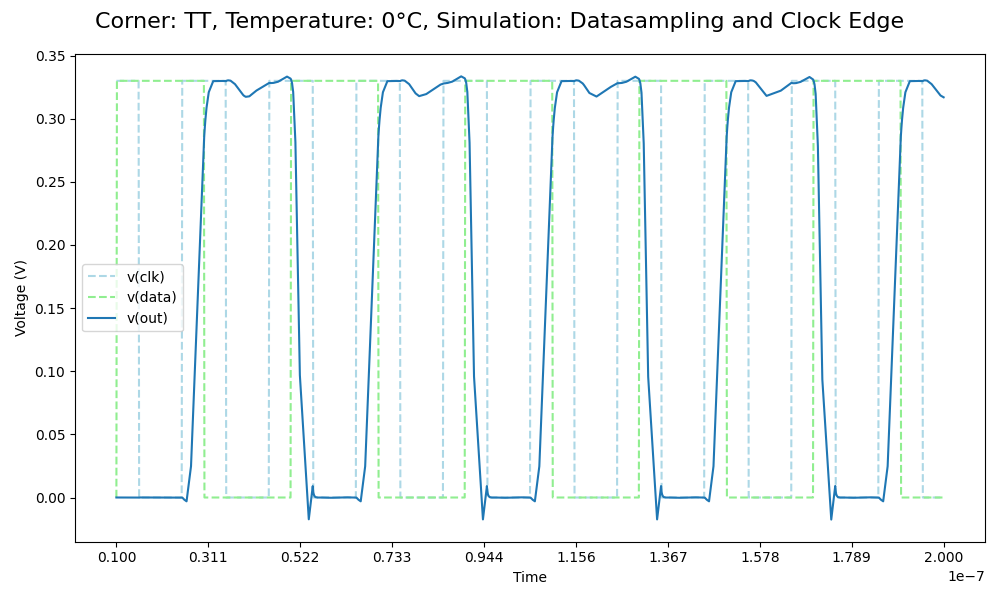
\includegraphics[height= 0.21\textheight]{figures/aimspice/TT/0/W1.csv.png}
    \vspace{5pt}
    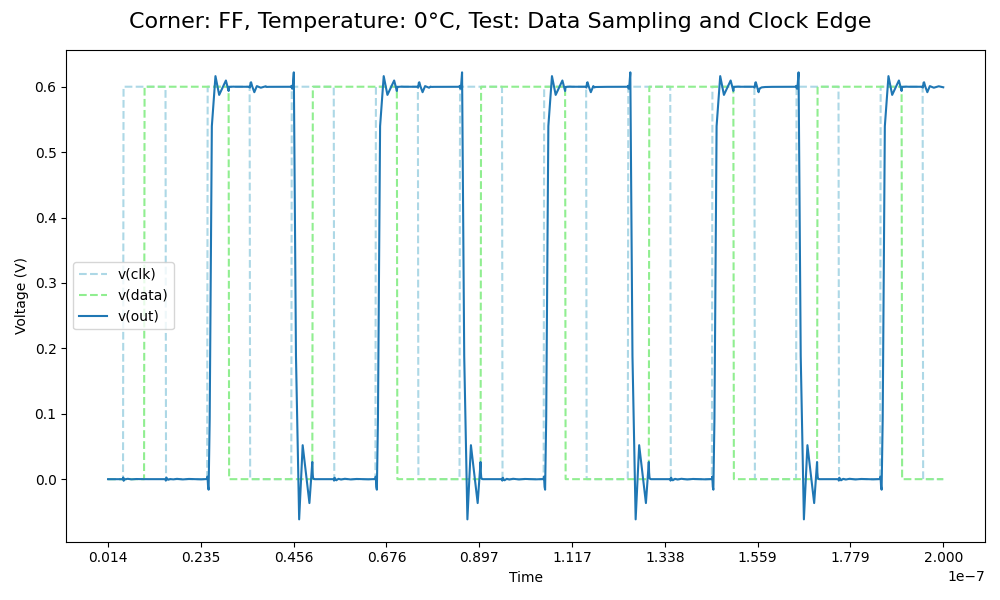
\includegraphics[height= 0.21\textheight]{figures/aimspice/FF/0/W1.csv.png}
    \vspace{5pt}
    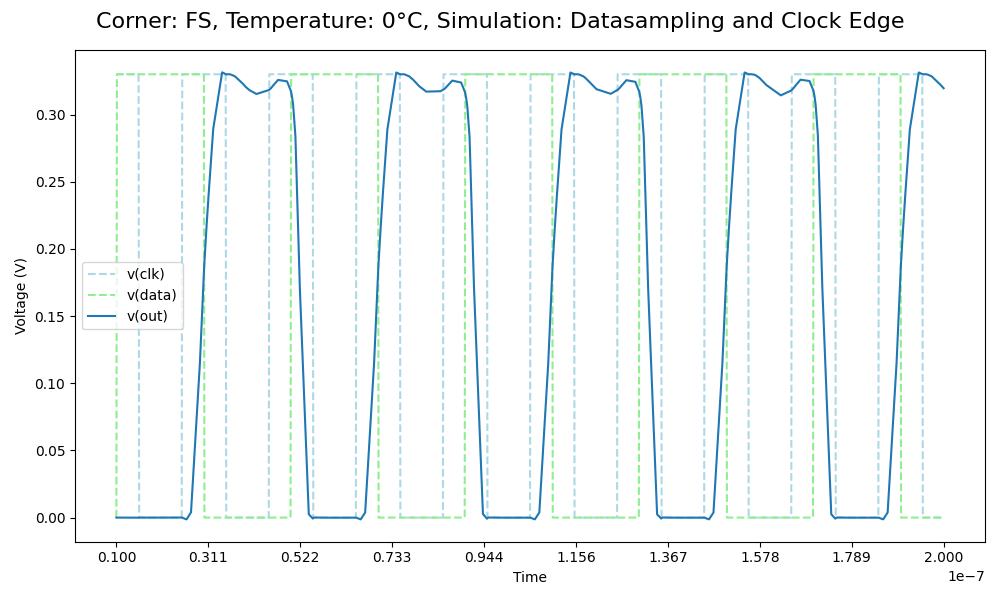
\includegraphics[height= 0.21\textheight]{figures/aimspice/FS/0/W1.csv.png}
    \vspace{5pt}
    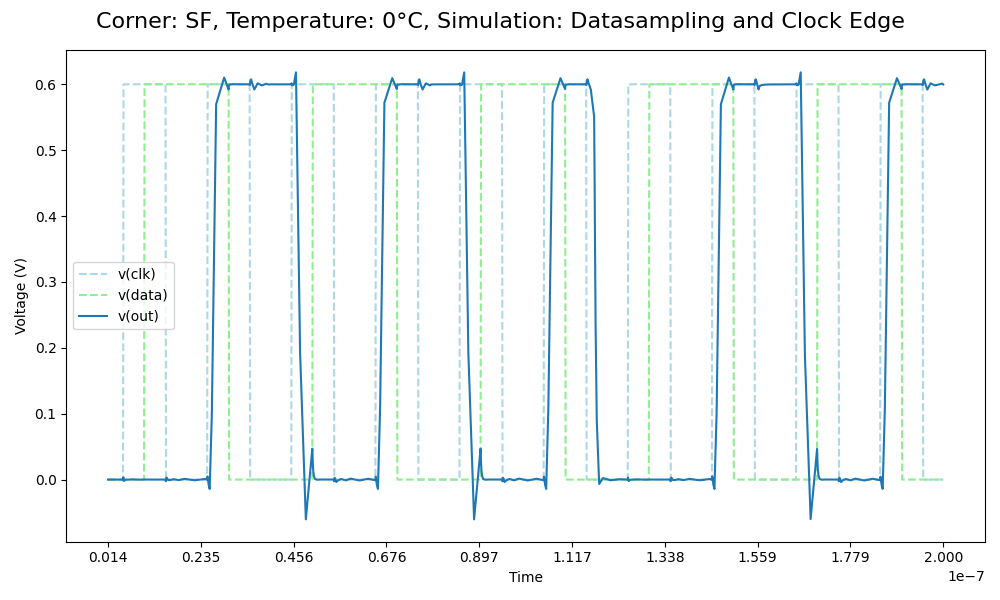
\includegraphics[height= 0.21\textheight]{figures/aimspice/SF/0/W1.csv.png}
    \vspace{5pt}
    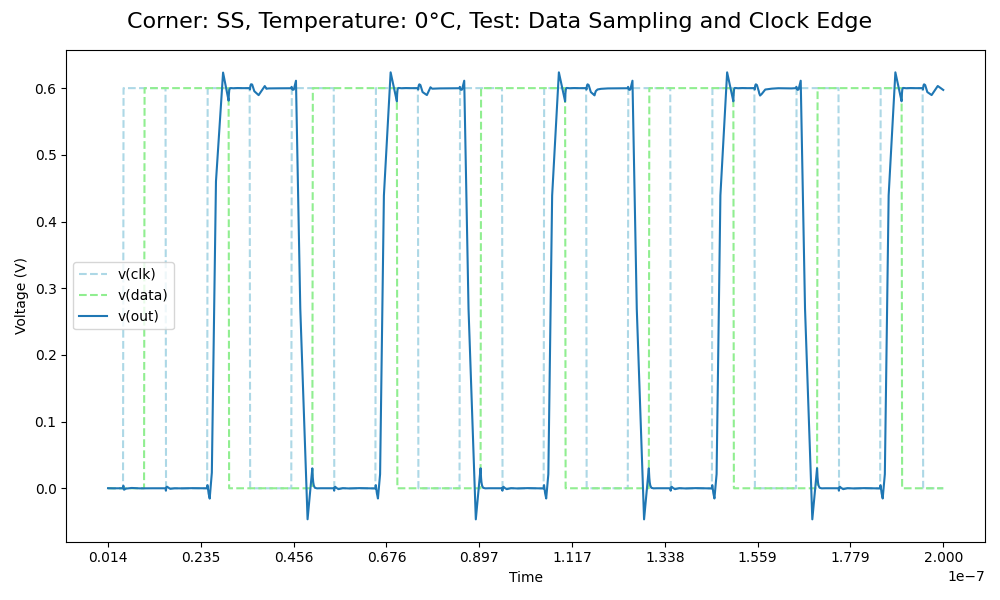
\includegraphics[height= 0.21\textheight]{figures/aimspice/SS/0/W1.csv.png}
    \caption{Simulation of datasampling at clock edge at 0 degrees Celsius.}
    \label{fig:aimspice_W1_0}
\end{figure}

\pagebreak

\begin{figure}[H]
    \centering
    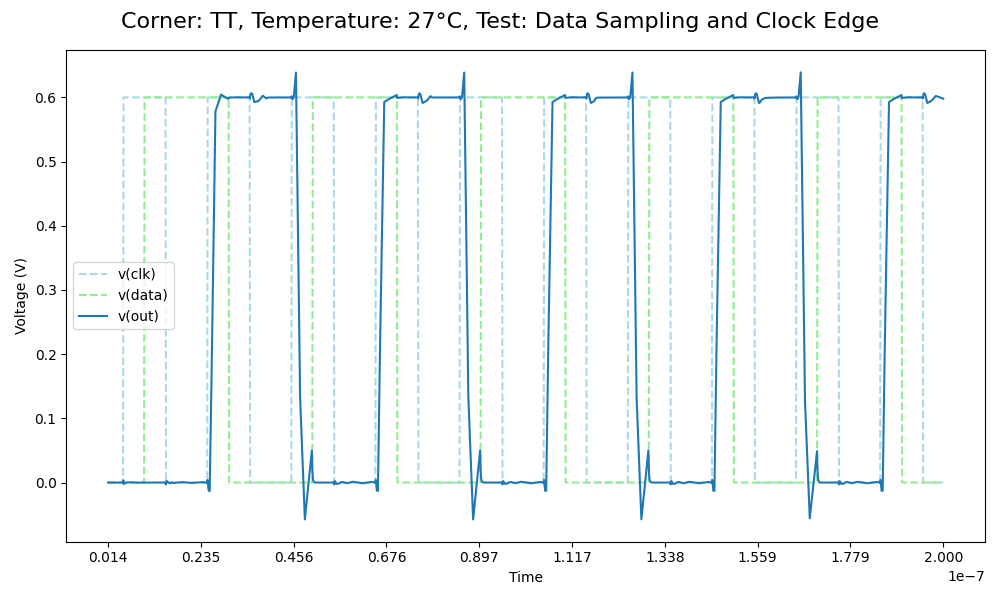
\includegraphics[height= 0.21\textheight]{figures/aimspice/TT/27/W1.csv.png}
    \vspace{5pt}
    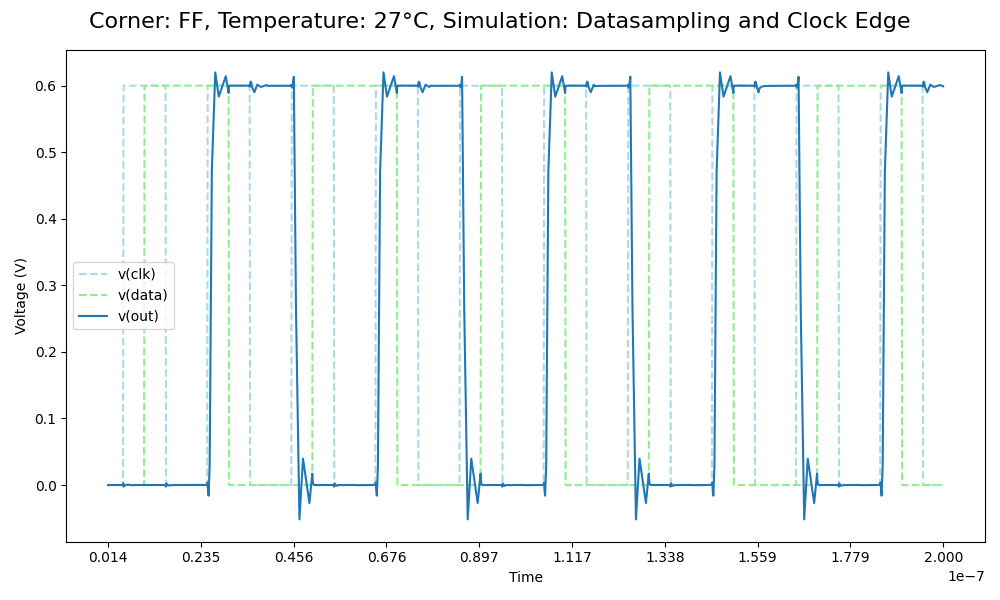
\includegraphics[height= 0.21\textheight]{figures/aimspice/FF/27/W1.csv.png}
    \vspace{5pt}
    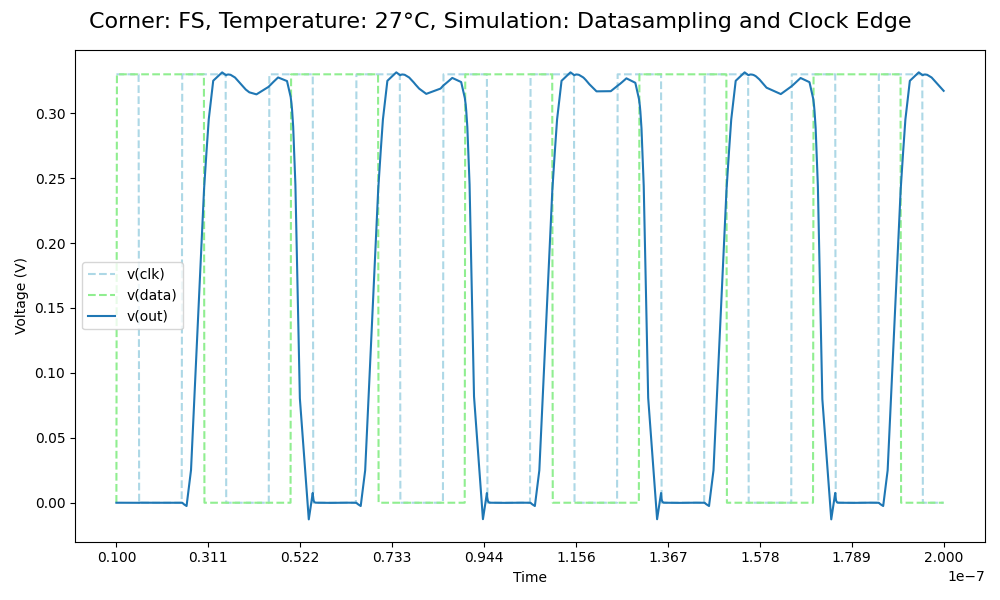
\includegraphics[height= 0.21\textheight]{figures/aimspice/FS/27/W1.csv.png}
    \vspace{5pt}
    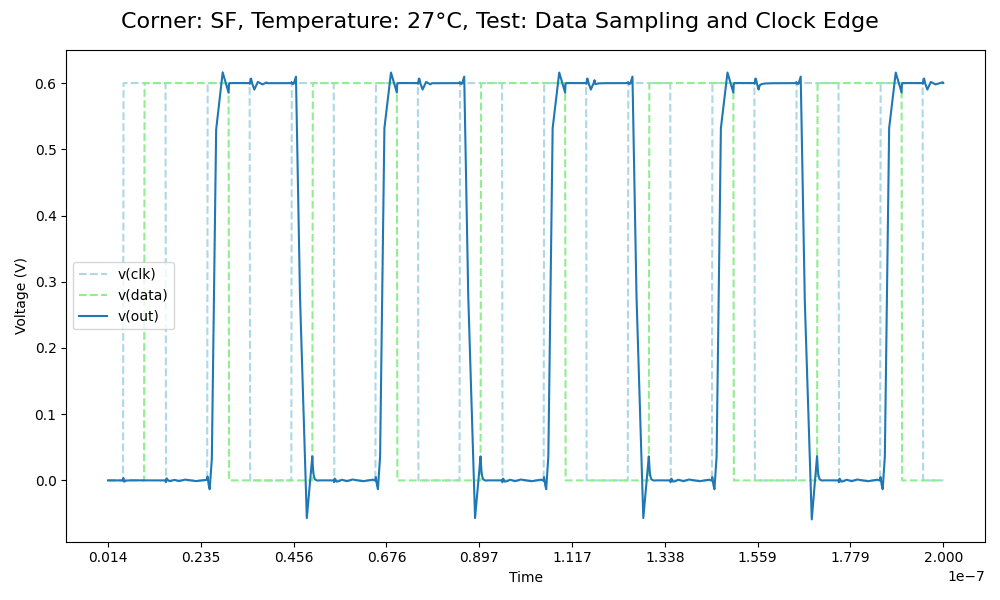
\includegraphics[height= 0.21\textheight]{figures/aimspice/SF/27/W1.csv.png}
    \vspace{5pt}
    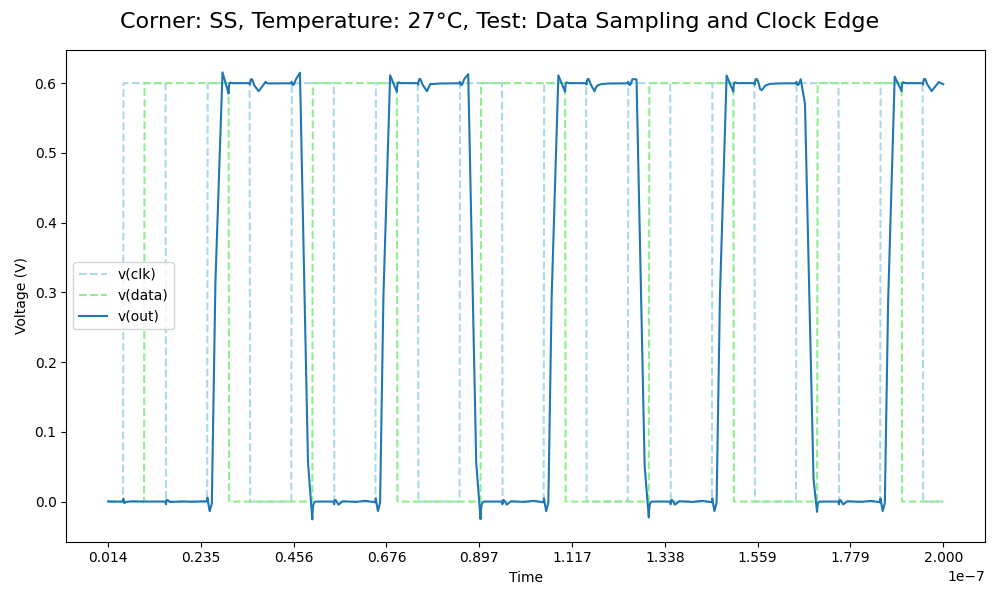
\includegraphics[height= 0.21\textheight]{figures/aimspice/SS/27/W1.csv.png}
    \caption{Simulation of datasampling at clock edge at 27 degrees Celsius.}
    \label{fig:aimspice_W1_27}
\end{figure}

\pagebreak

\begin{figure}[H]
    \centering
    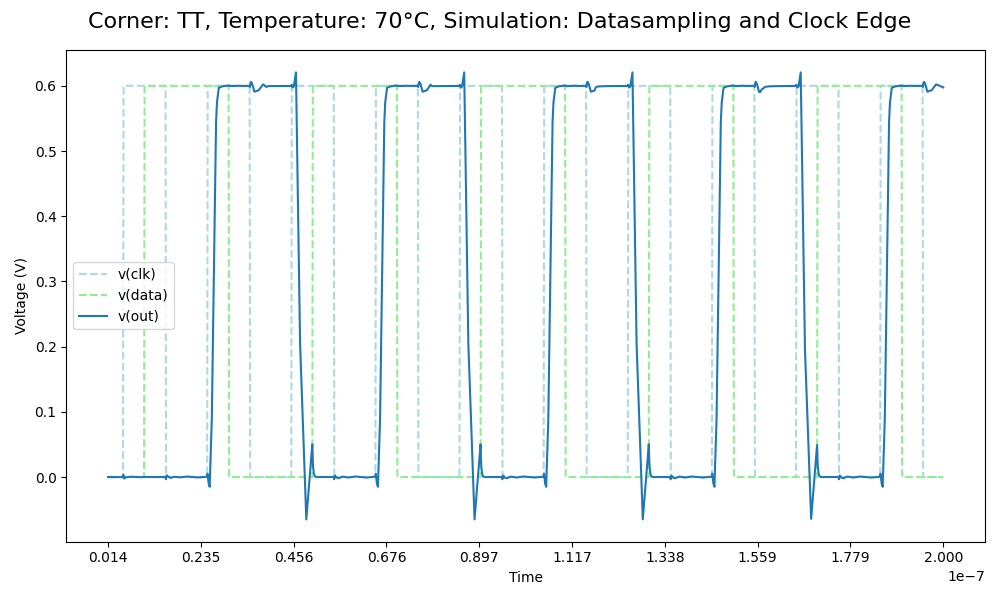
\includegraphics[height= 0.21\textheight]{figures/aimspice/TT/70/W1.csv.png}
    \vspace{5pt}
    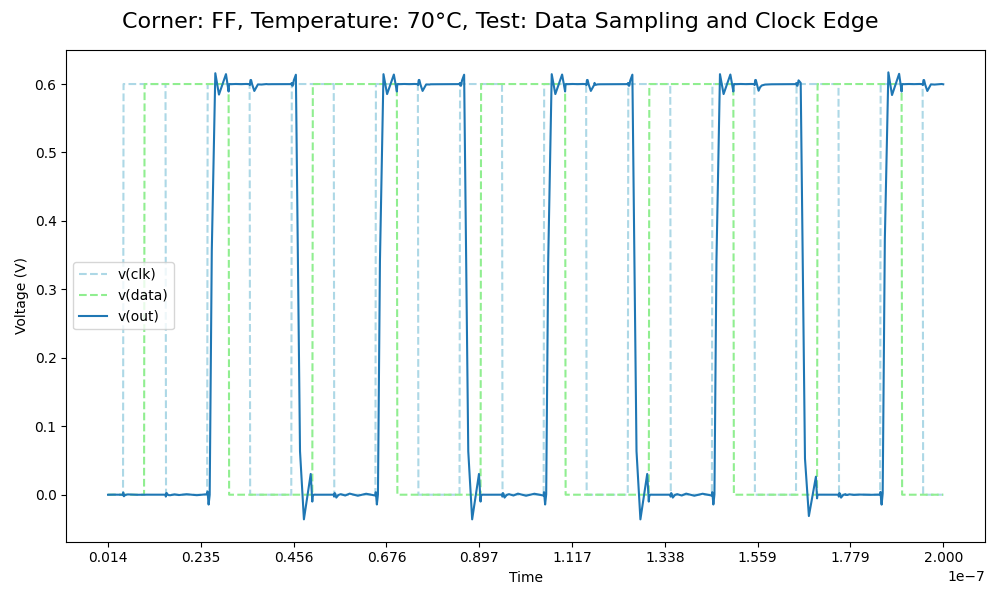
\includegraphics[height= 0.21\textheight]{figures/aimspice/FF/70/W1.csv.png}
    \vspace{5pt}
    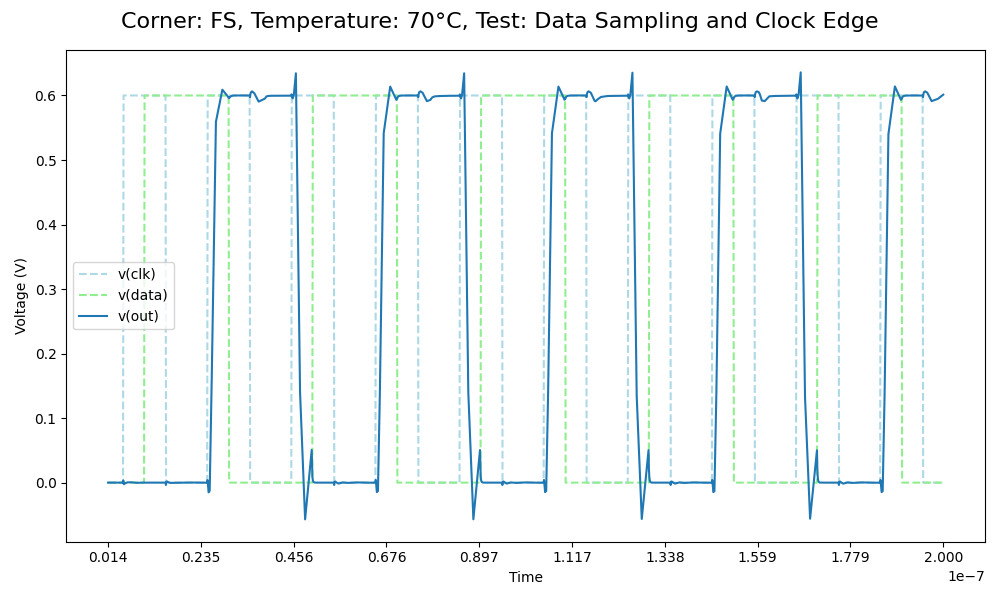
\includegraphics[height= 0.21\textheight]{figures/aimspice/FS/70/W1.csv.png}
    \vspace{5pt}
    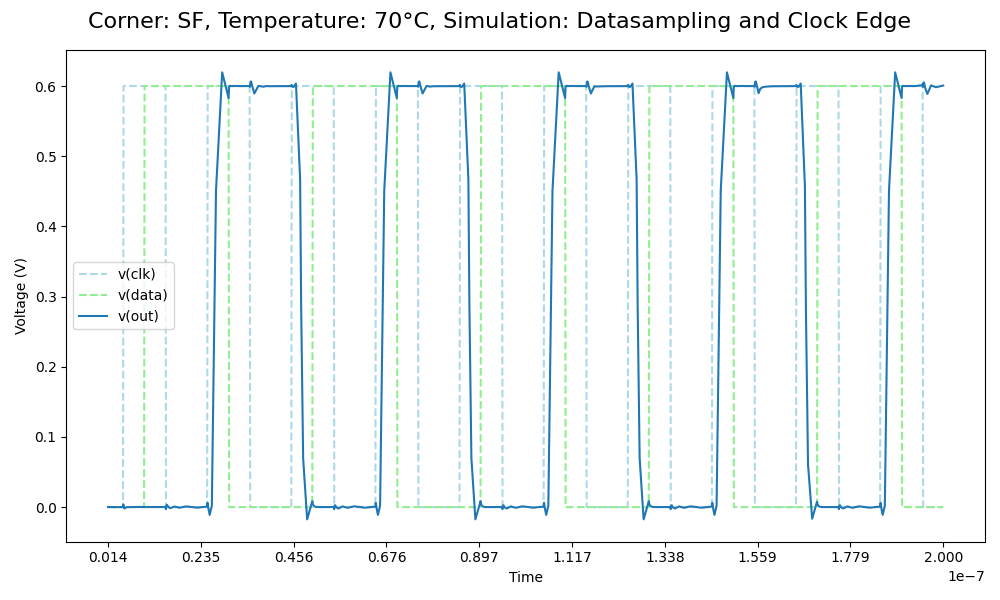
\includegraphics[height= 0.21\textheight]{figures/aimspice/SF/70/W1.csv.png}
    \vspace{5pt}
    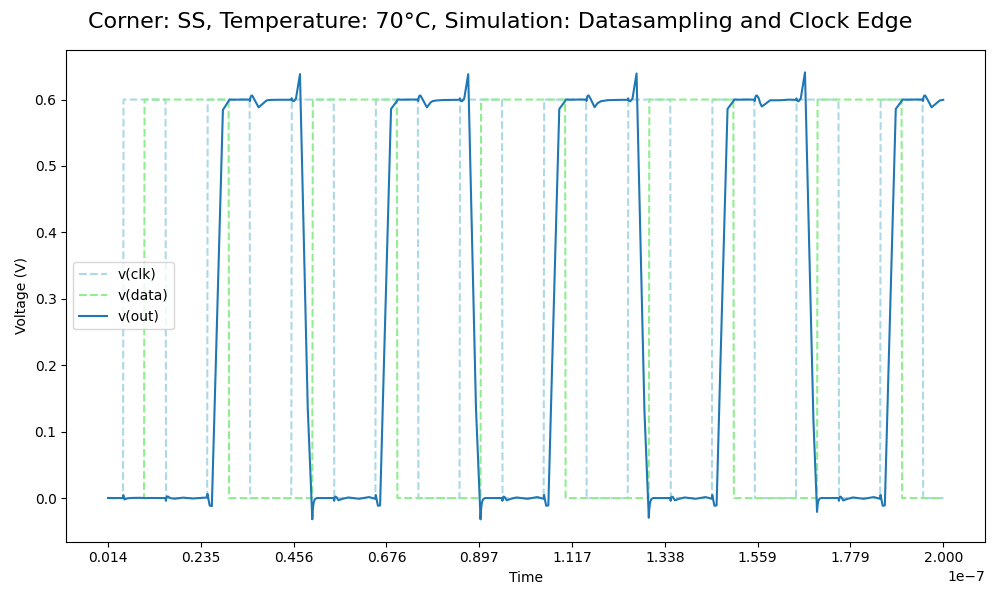
\includegraphics[height= 0.21\textheight]{figures/aimspice/SS/70/W1.csv.png}
    \caption{Simulation of datasampling at clock edge at 70 degrees Celsius.}
    \label{fig:aimspice_W1_70}
\end{figure}

\pagebreak

\begin{figure}[H]
    \centering
    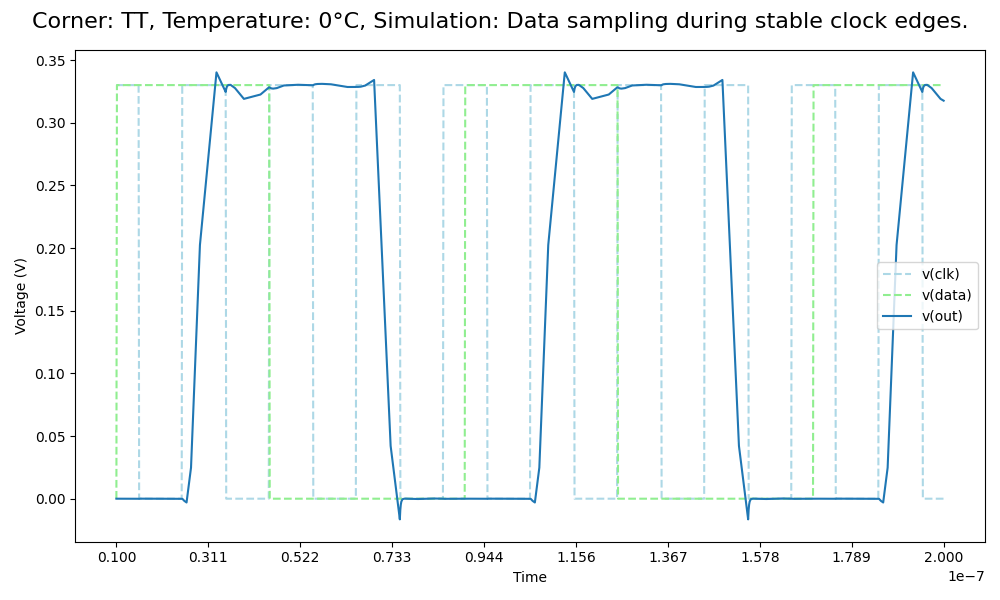
\includegraphics[height= 0.21\textheight]{figures/aimspice/TT/0/W2.csv.png}
    \vspace{5pt}
    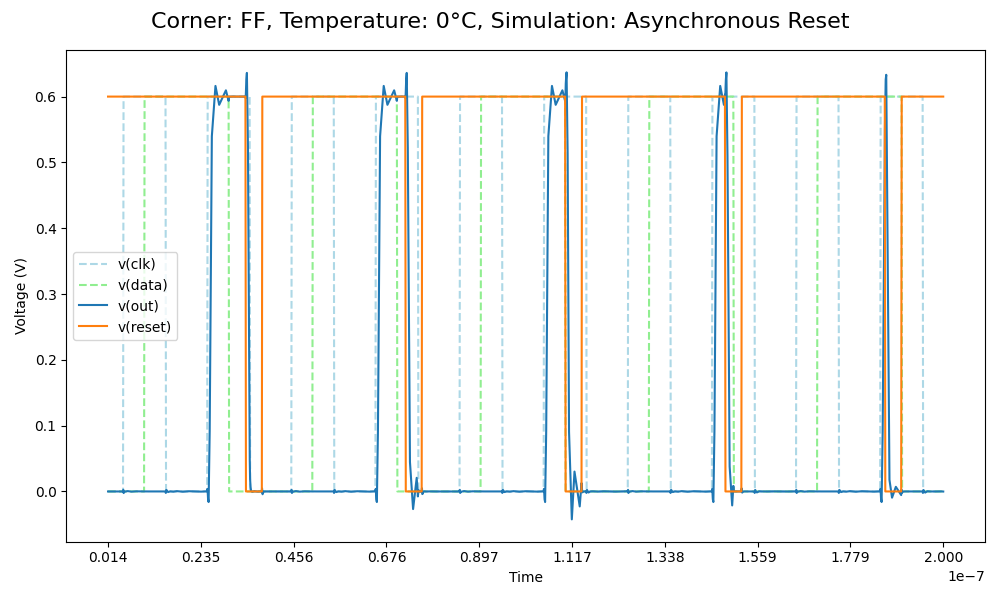
\includegraphics[height= 0.21\textheight]{figures/aimspice/FF/0/W2.csv.png}
    \vspace{5pt}
    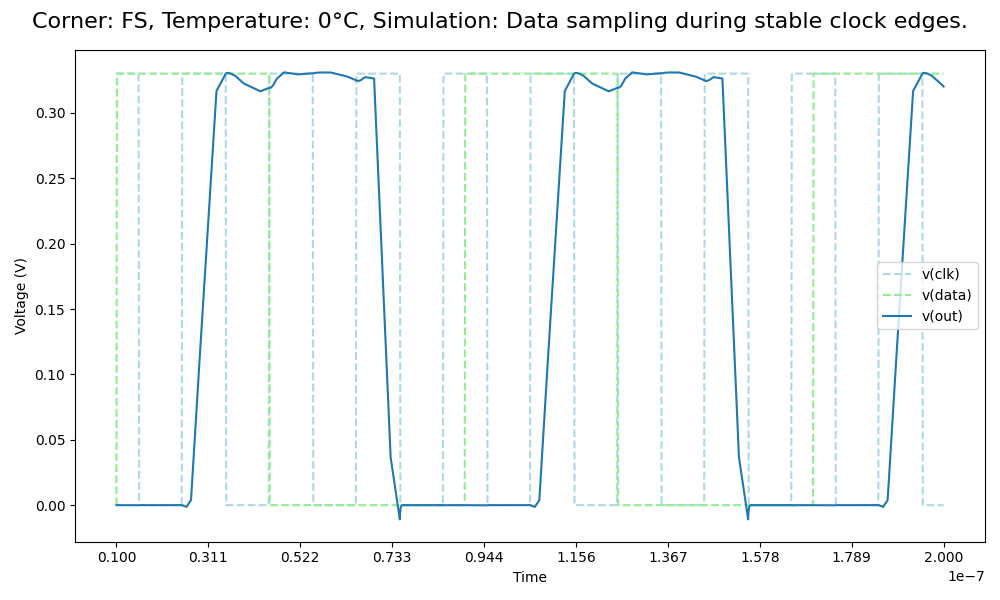
\includegraphics[height= 0.21\textheight]{figures/aimspice/FS/0/W2.csv.png}
    \vspace{5pt}
    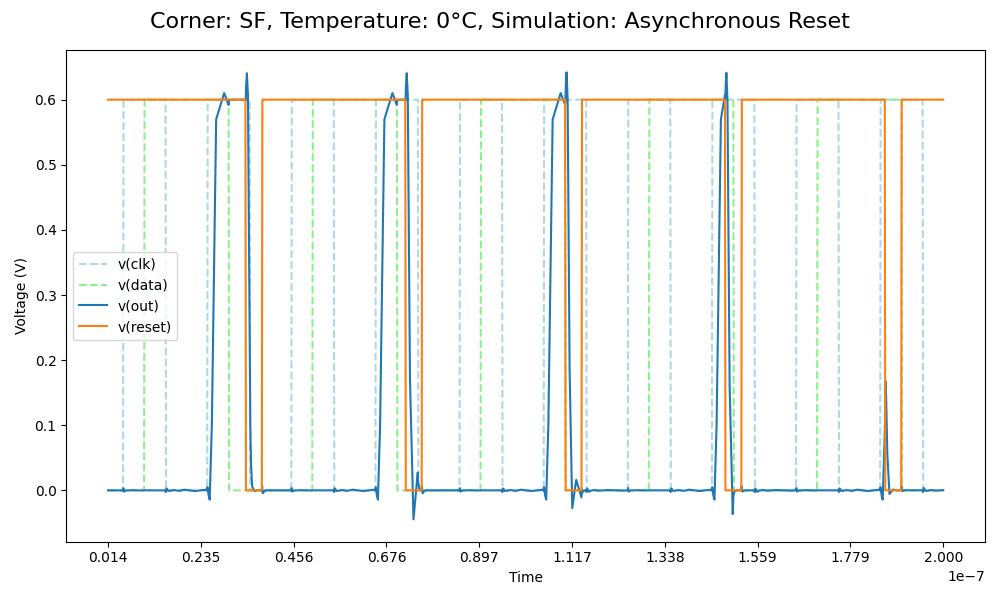
\includegraphics[height= 0.21\textheight]{figures/aimspice/SF/0/W2.csv.png}
    \vspace{5pt}
    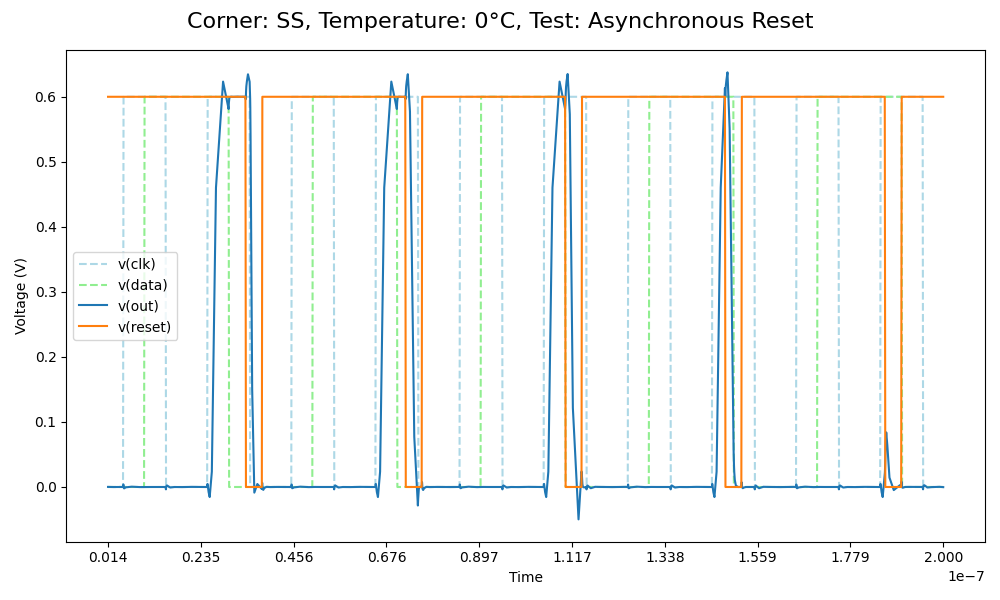
\includegraphics[height= 0.21\textheight]{figures/aimspice/SS/0/W2.csv.png}
    \caption{Simulation of datasampling when the data stays the same for a few clock edges at 0 degrees celcius.}
    \label{fig:aimspice_W2_0}
\end{figure}

\pagebreak

\begin{figure}[H]
    \centering
    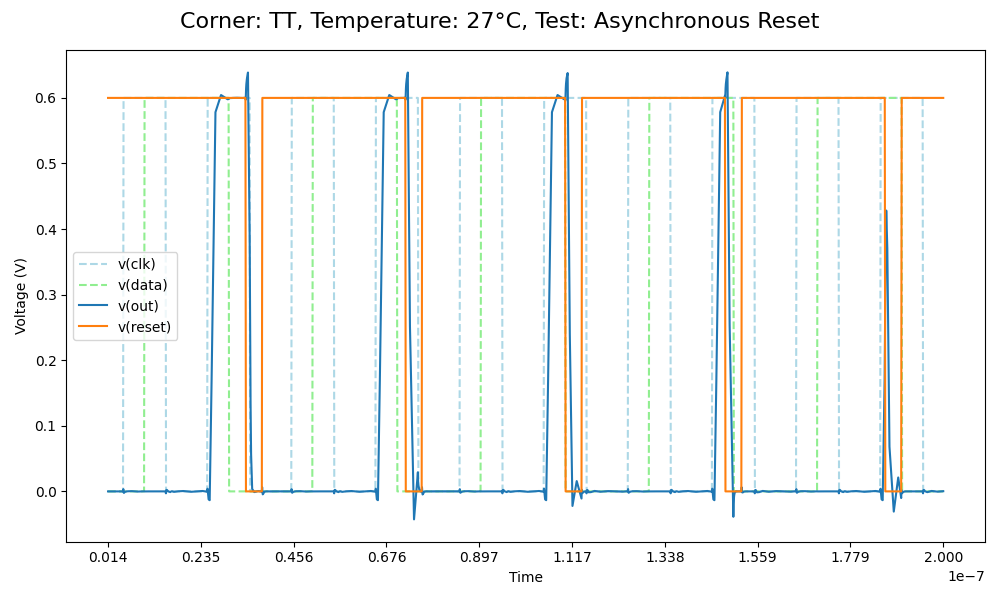
\includegraphics[height= 0.21\textheight]{figures/aimspice/TT/27/W2.csv.png}
    \vspace{5pt}
    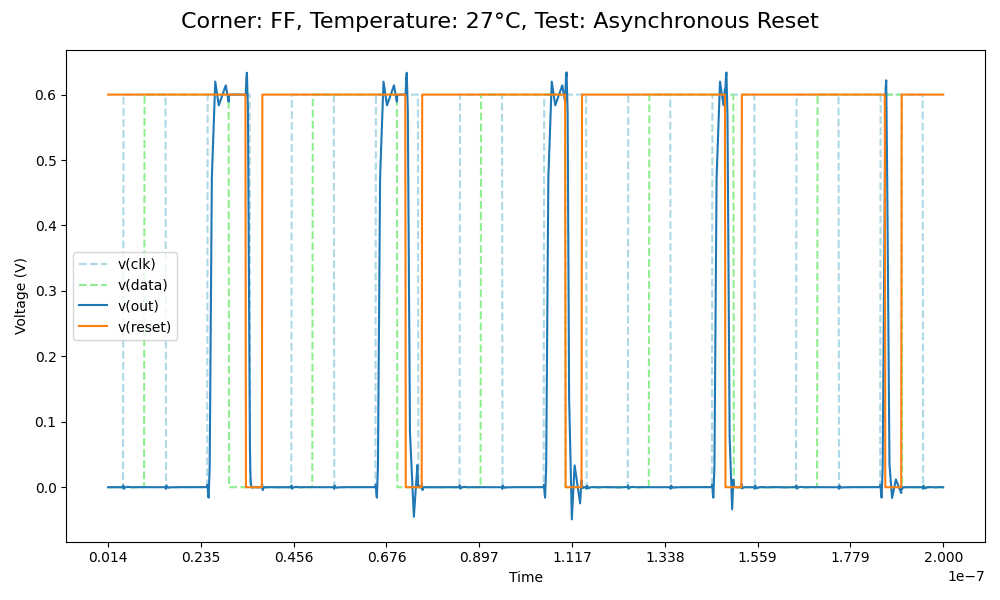
\includegraphics[height= 0.21\textheight]{figures/aimspice/FF/27/W2.csv.png}
    \vspace{5pt}
    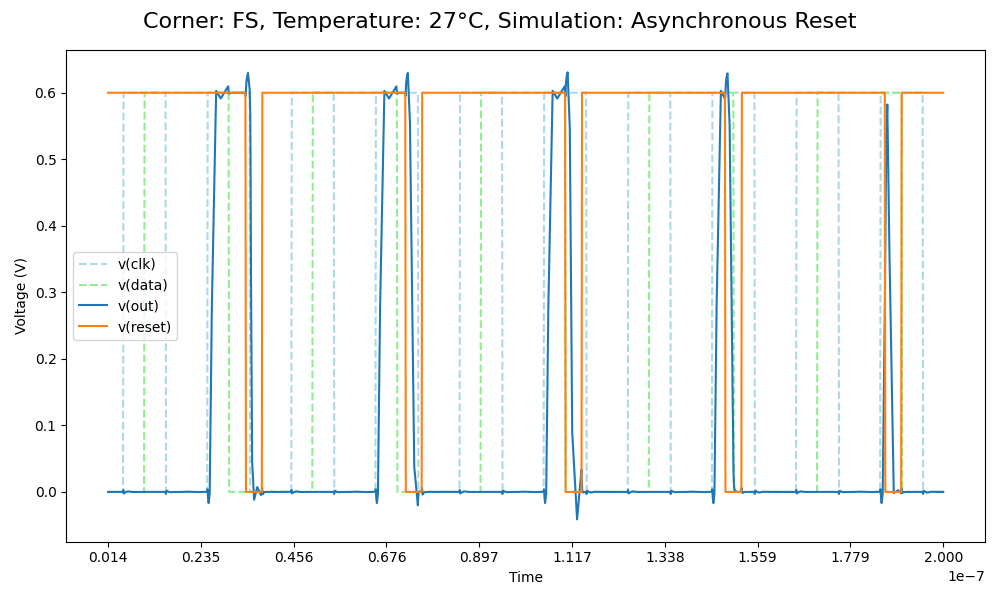
\includegraphics[height= 0.21\textheight]{figures/aimspice/FS/27/W2.csv.png}
    \vspace{5pt}
    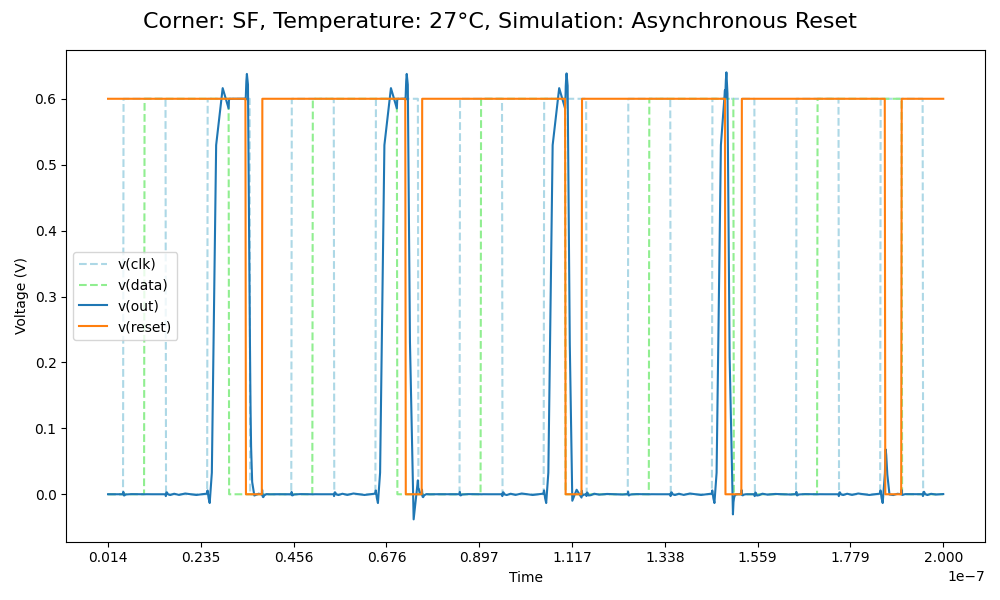
\includegraphics[height= 0.21\textheight]{figures/aimspice/SF/27/W2.csv.png}
    \vspace{5pt}
    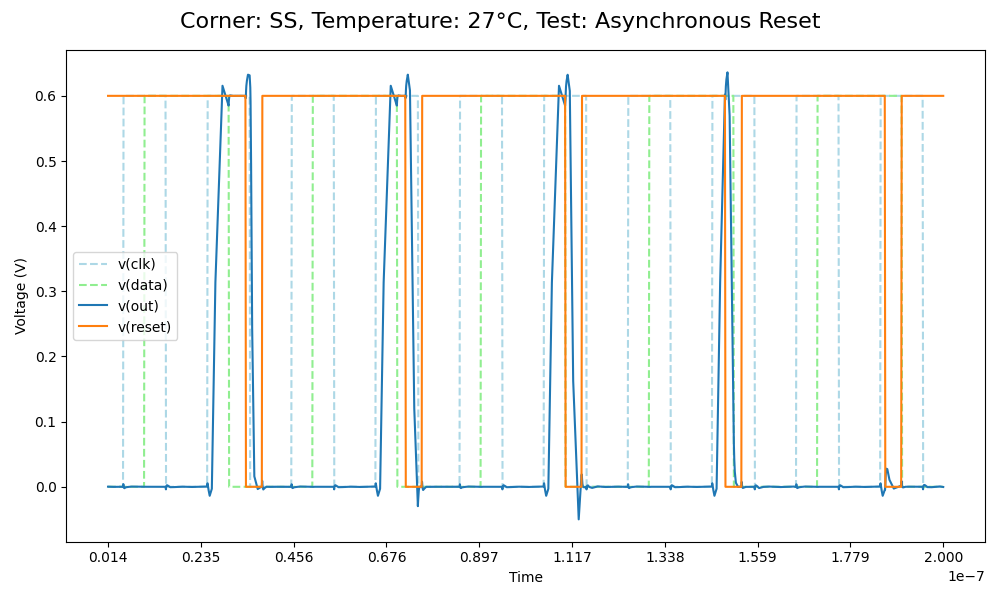
\includegraphics[height= 0.21\textheight]{figures/aimspice/SS/27/W2.csv.png}
    \caption{Simulation of datasampling when the data stays the same for a few clock edges at 27 degrees celcius.}
    \label{fig:aimspice_W2_27}
\end{figure}

\pagebreak

\begin{figure}[H]
    \centering
    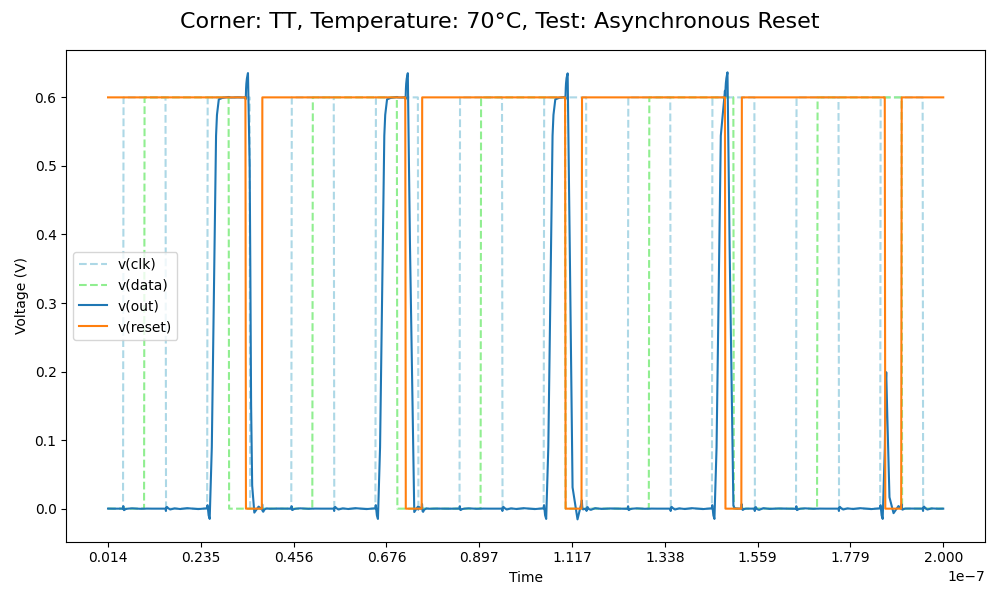
\includegraphics[height= 0.21\textheight]{figures/aimspice/TT/70/W2.csv.png}
    \vspace{5pt}
    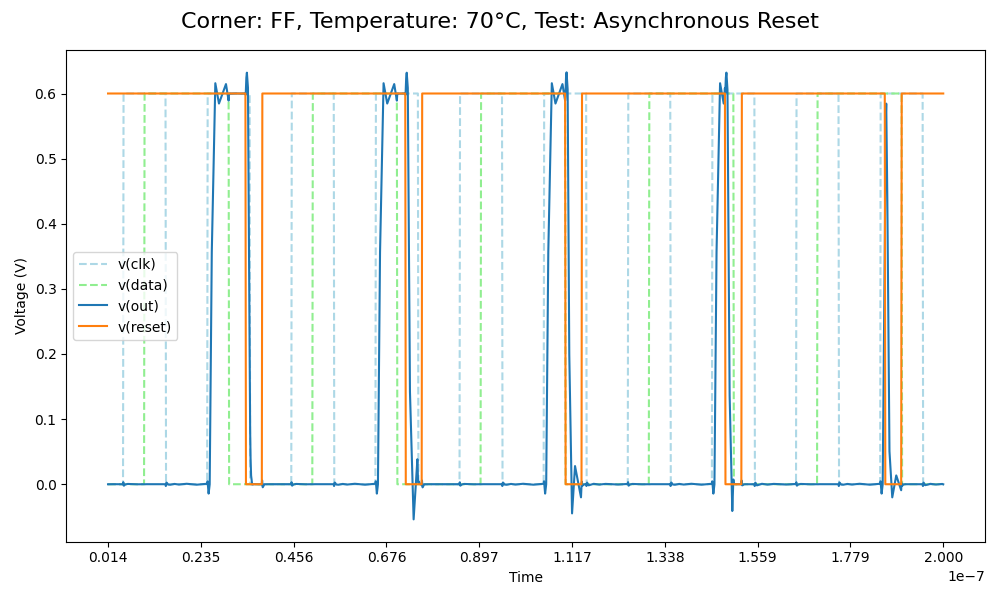
\includegraphics[height= 0.21\textheight]{figures/aimspice/FF/70/W2.csv.png}
    \vspace{5pt}
    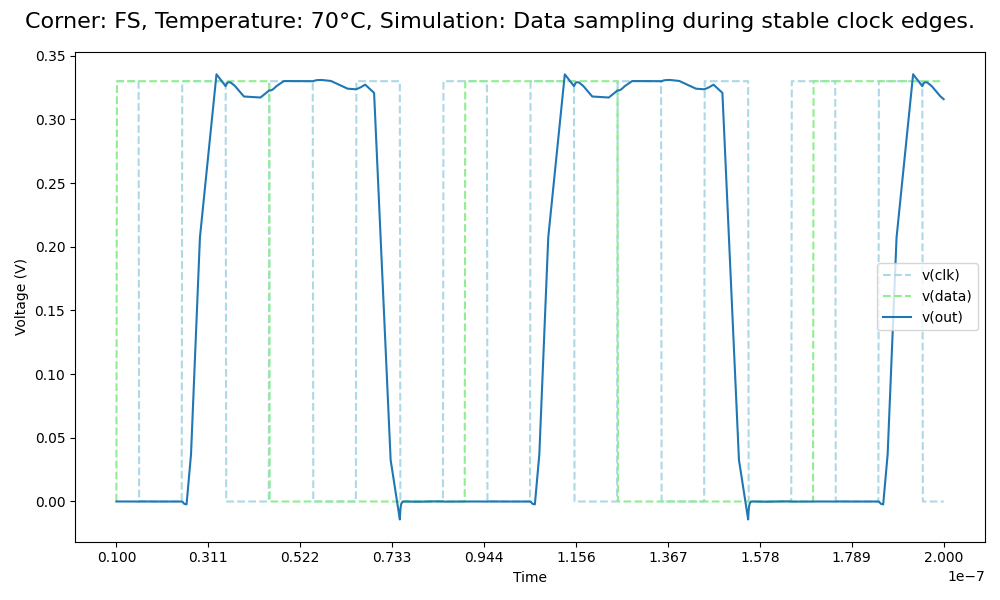
\includegraphics[height= 0.21\textheight]{figures/aimspice/FS/70/W2.csv.png}
    \vspace{5pt}
    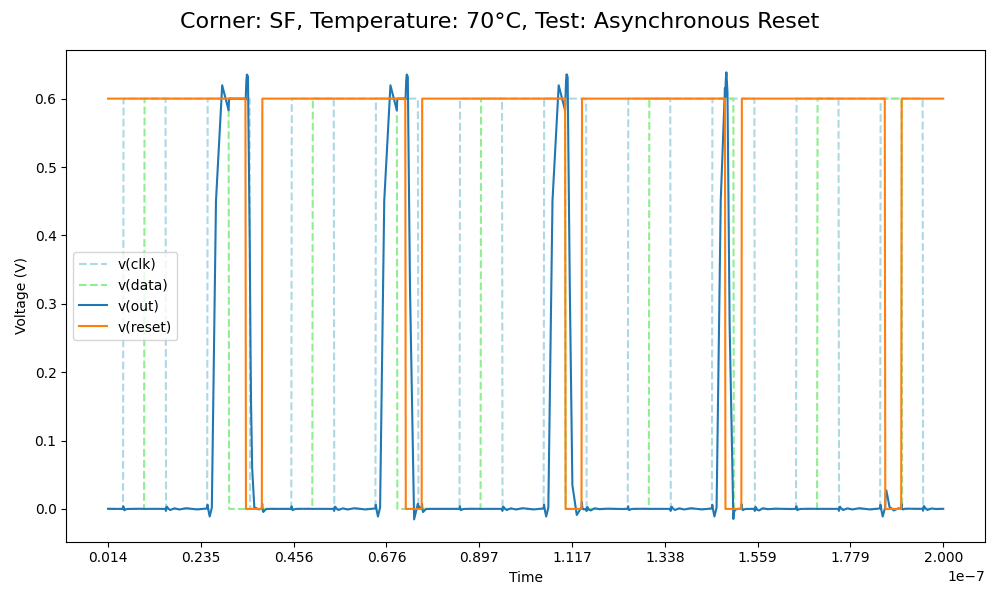
\includegraphics[height= 0.21\textheight]{figures/aimspice/SF/70/W2.csv.png}
    \vspace{5pt}
    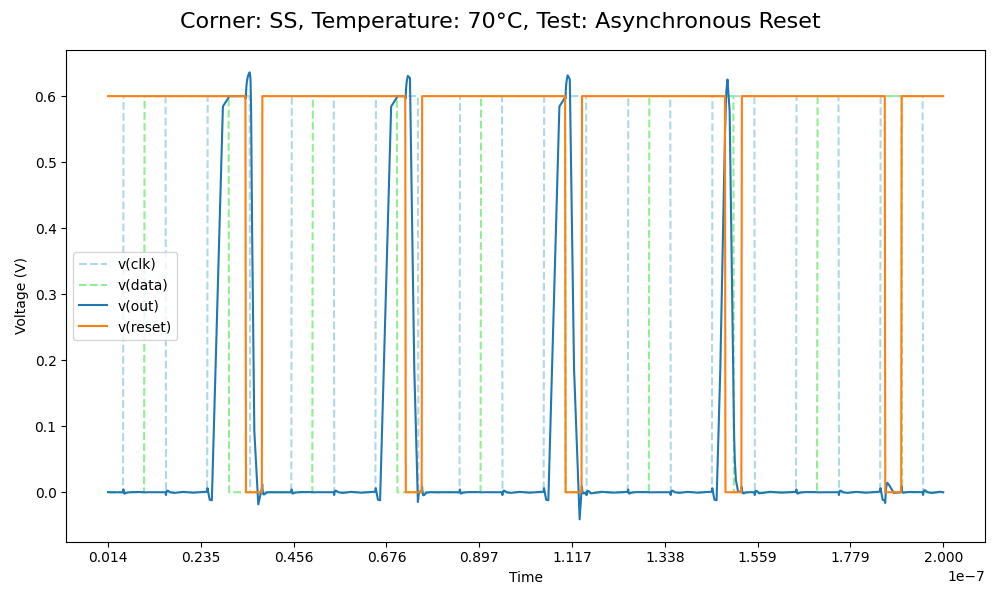
\includegraphics[height= 0.21\textheight]{figures/aimspice/SS/70/W2.csv.png}
    \caption{Simulation of datasampling when the data stays the same for a few clock edges at 70 degrees celcius.}
    \label{fig:aimspice_W2_70}
\end{figure}

\pagebreak

\pagebreak

\begin{figure}[H]
    \centering
    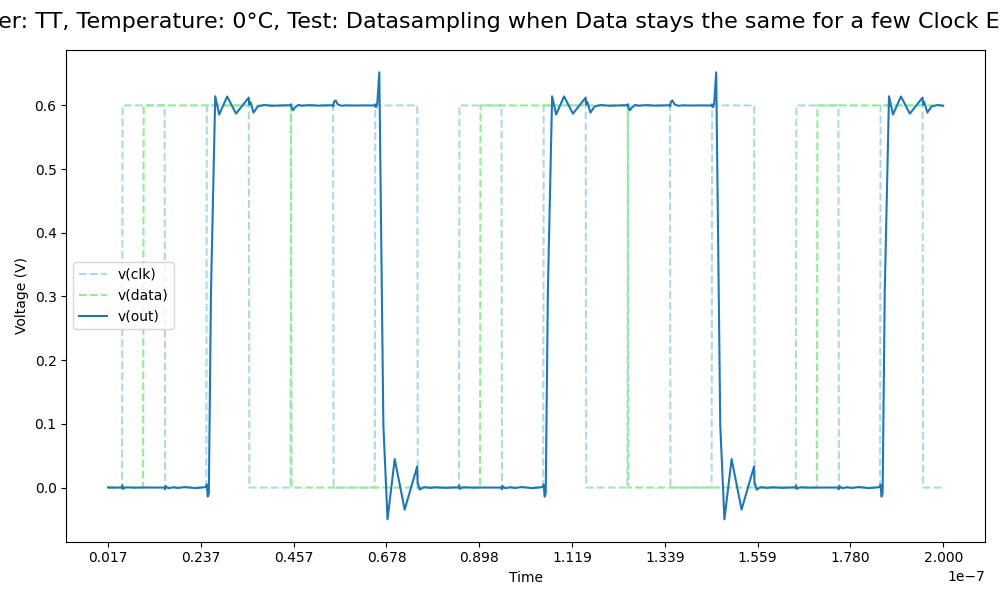
\includegraphics[height= 0.21\textheight]{figures/aimspice/TT/0/W3.csv.png}
    \vspace{5pt}
    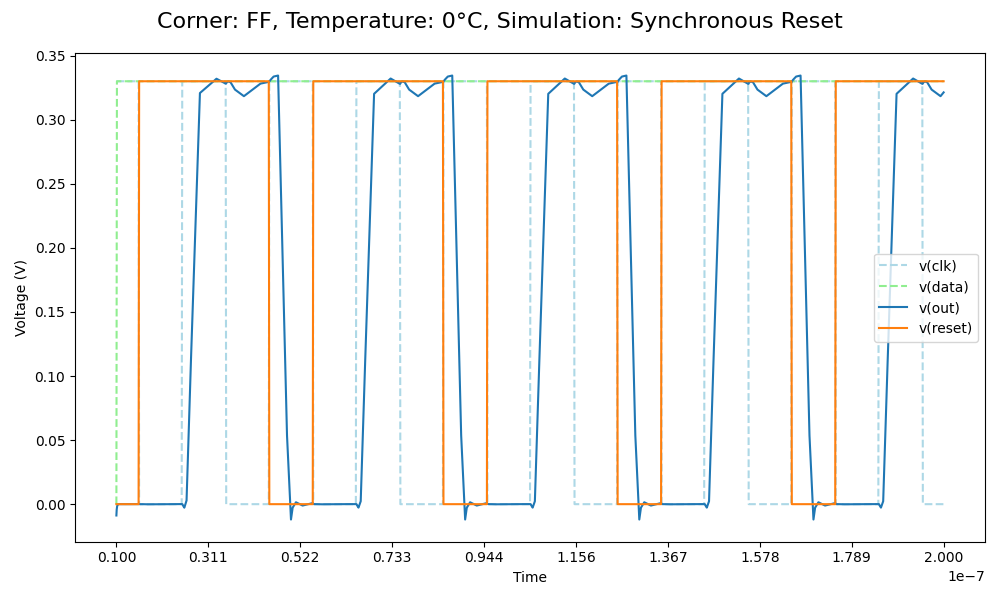
\includegraphics[height= 0.21\textheight]{figures/aimspice/FF/0/W3.csv.png}
    \vspace{5pt}
    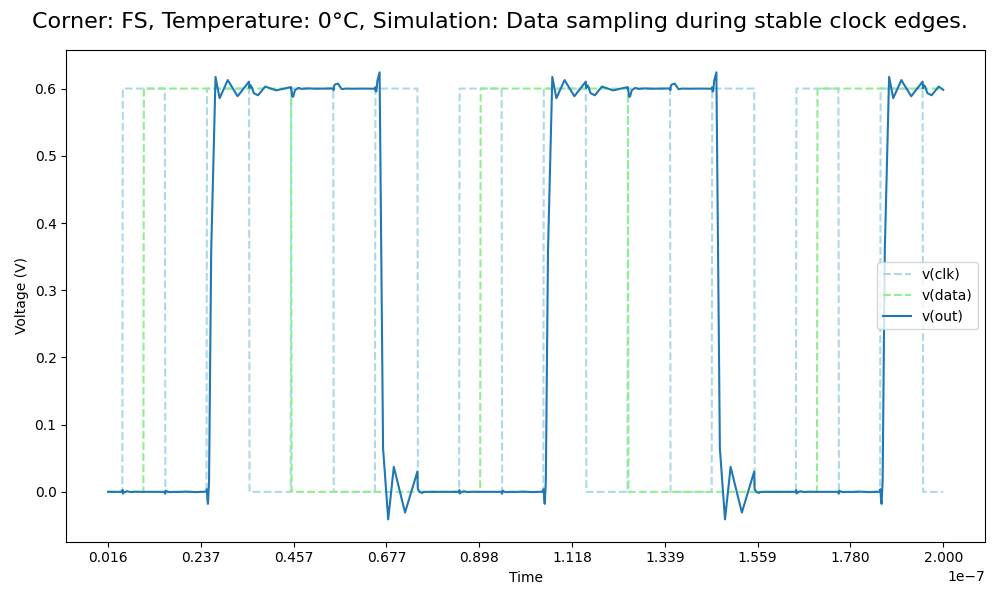
\includegraphics[height= 0.21\textheight]{figures/aimspice/FS/0/W3.csv.png}
    \vspace{5pt}
    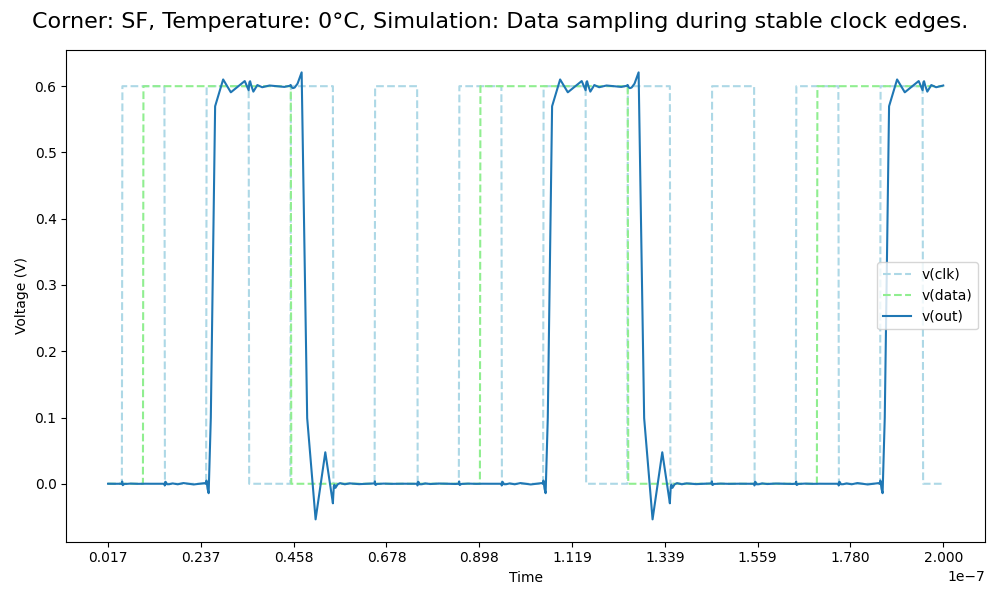
\includegraphics[height= 0.21\textheight]{figures/aimspice/SF/0/W3.csv.png}
    \vspace{5pt}
    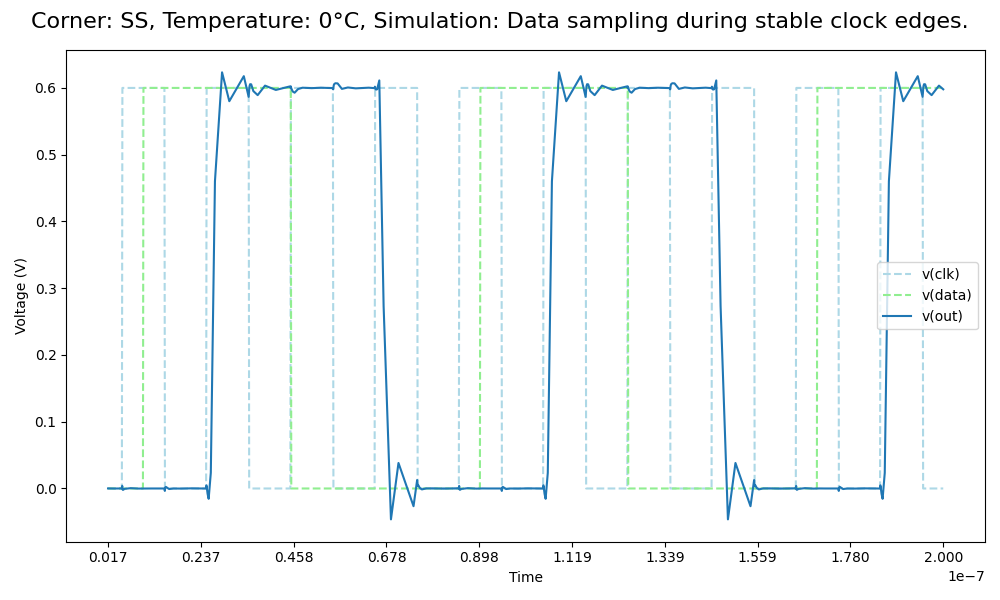
\includegraphics[height= 0.21\textheight]{figures/aimspice/SS/0/W3.csv.png}
    \caption{Simulation of the asynchronous reset at 0 degrees celcius.}
    \label{fig:aimspice_W3_0}
\end{figure}

\pagebreak

\begin{figure}[H]
    \centering
    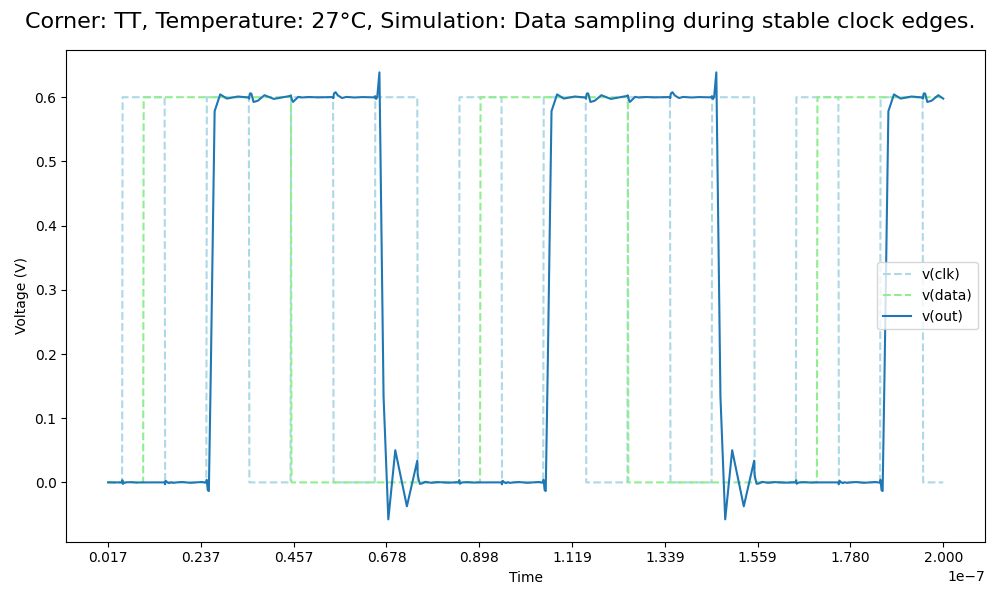
\includegraphics[height= 0.21\textheight]{figures/aimspice/TT/27/W3.csv.png}
    \vspace{5pt}
    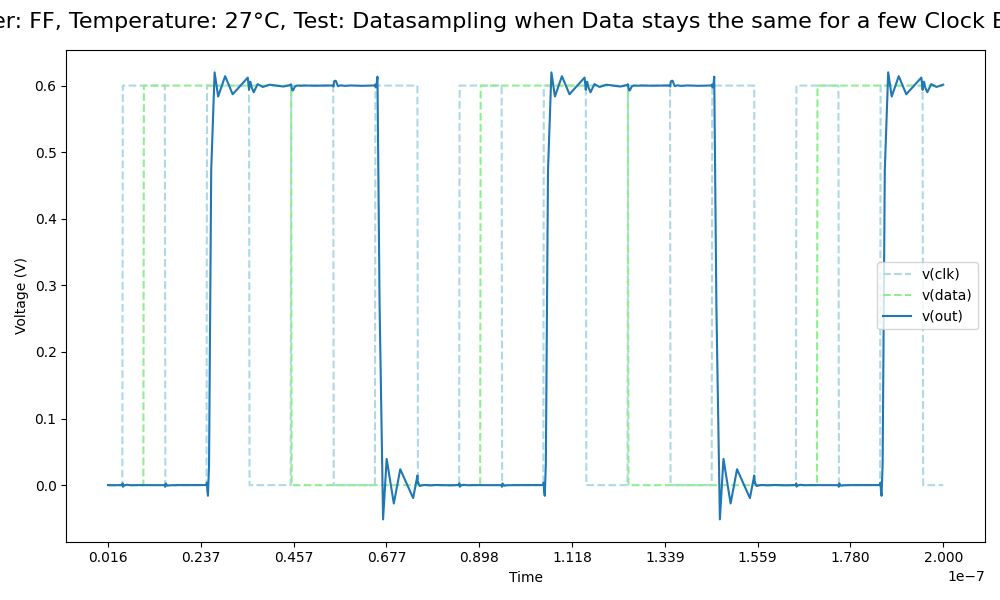
\includegraphics[height= 0.21\textheight]{figures/aimspice/FF/27/W3.csv.png}
    \vspace{5pt}
    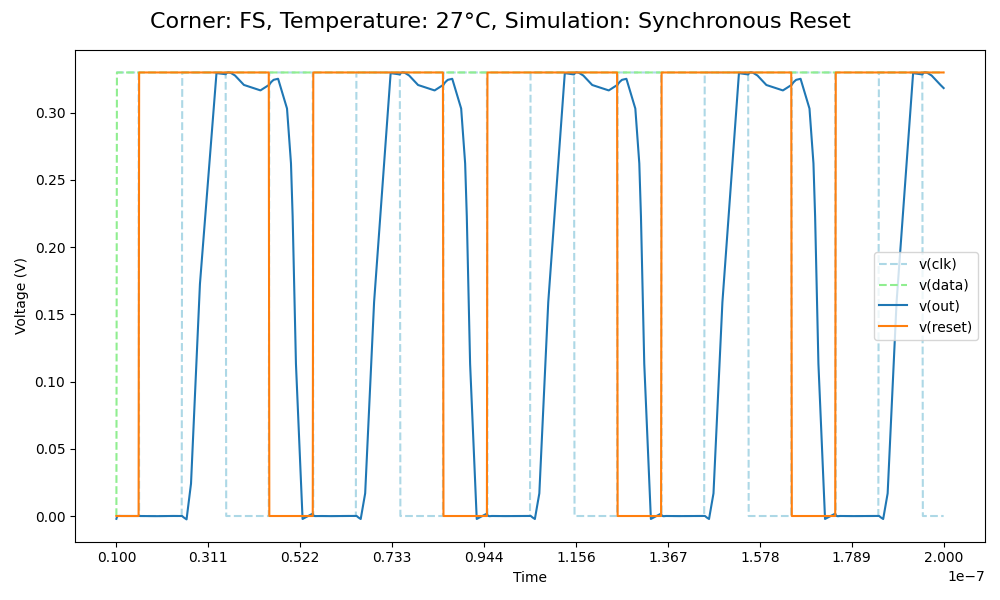
\includegraphics[height= 0.21\textheight]{figures/aimspice/FS/27/W3.csv.png}
    \vspace{5pt}
    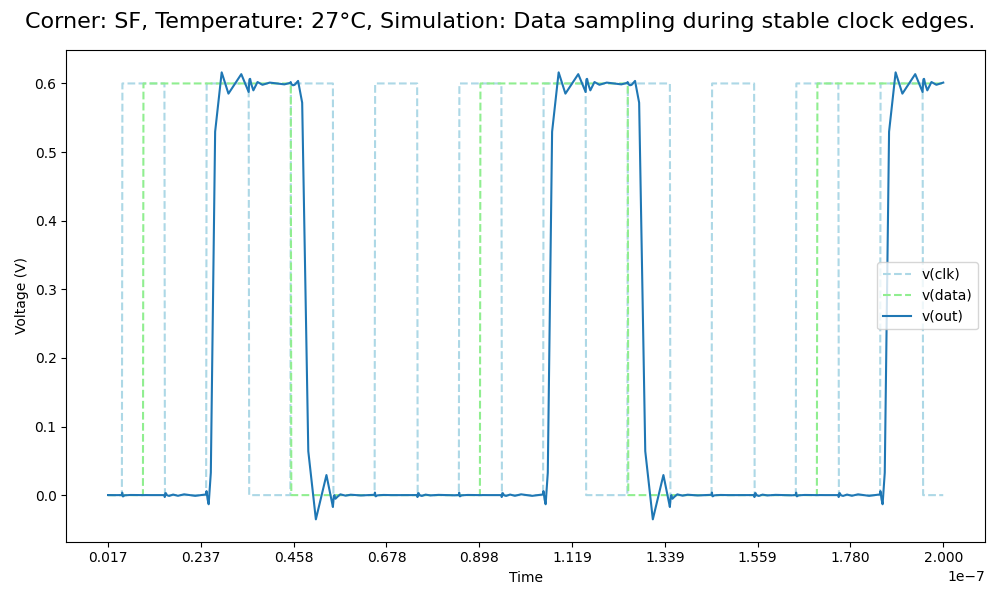
\includegraphics[height= 0.21\textheight]{figures/aimspice/SF/27/W3.csv.png}
    \vspace{5pt}
    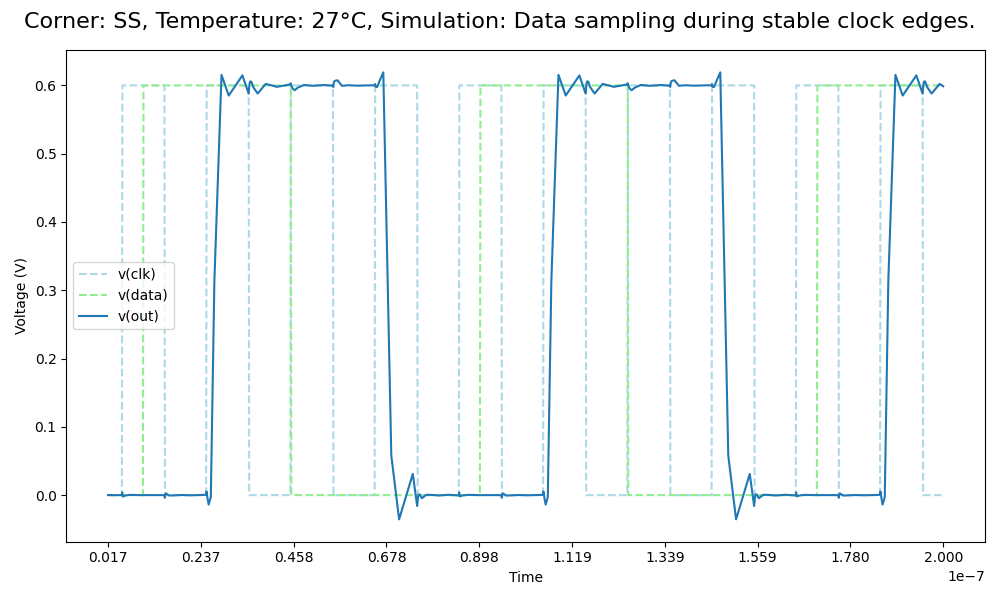
\includegraphics[height= 0.21\textheight]{figures/aimspice/SS/27/W3.csv.png}
    \caption{Simulation of the asynchronous reset at 27 degrees celcius.}
    \label{fig:aimspice_W3_27}
\end{figure}

\pagebreak

\begin{figure}[H]
    \centering
    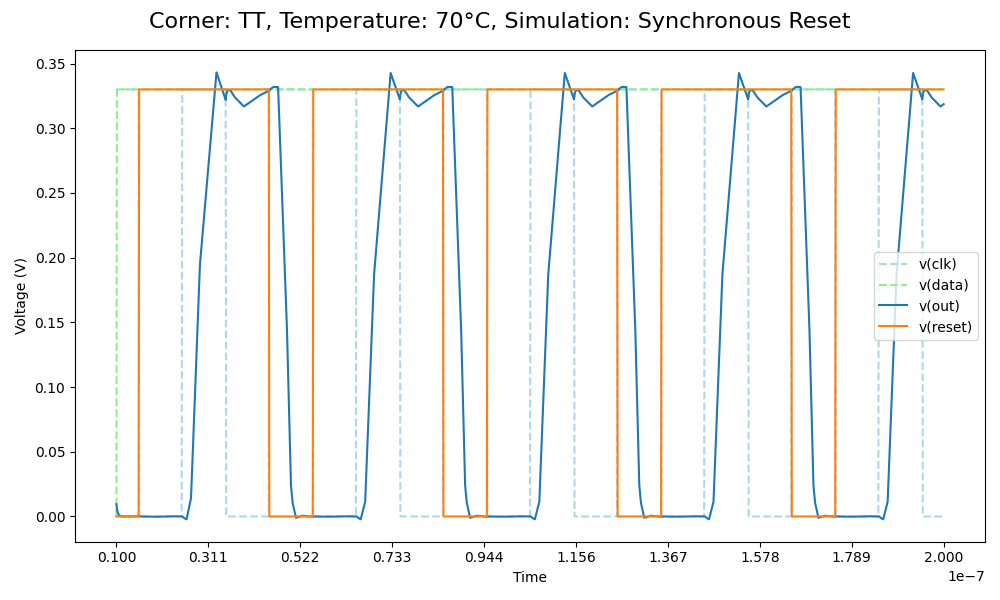
\includegraphics[height= 0.21\textheight]{figures/aimspice/TT/70/W3.csv.png}
    \vspace{5pt}
    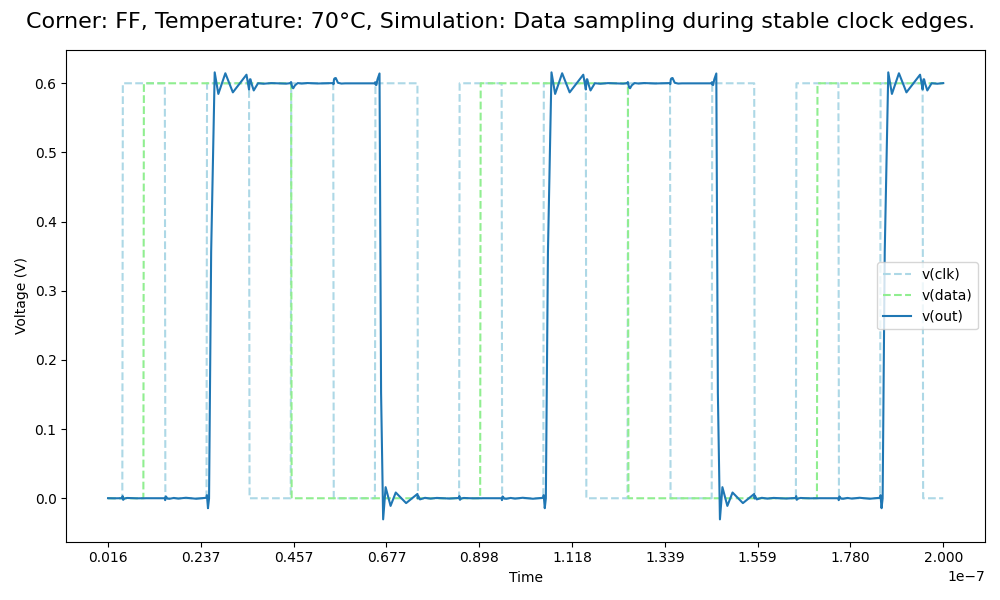
\includegraphics[height= 0.21\textheight]{figures/aimspice/FF/70/W3.csv.png}
    \vspace{5pt}
    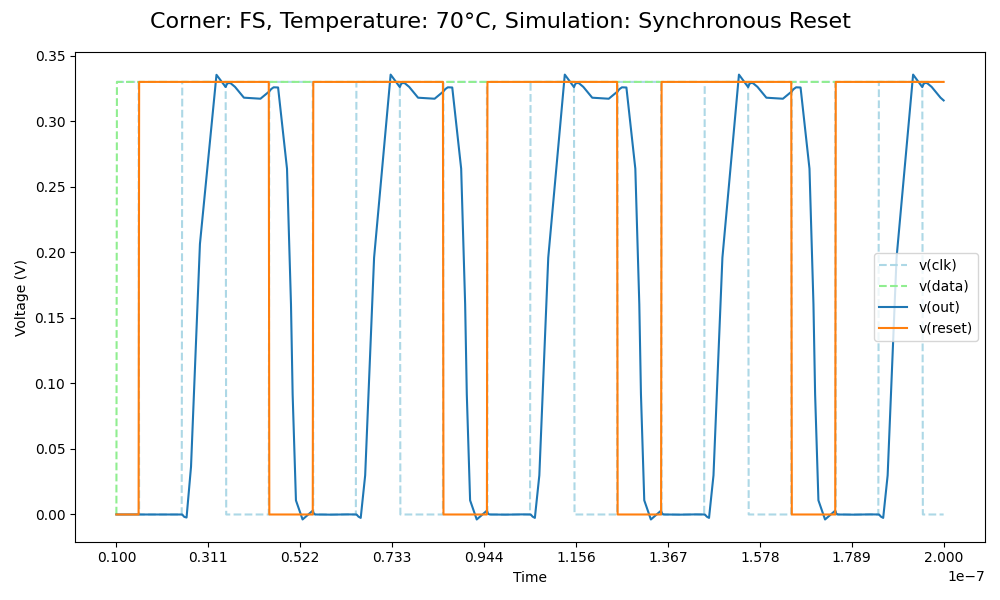
\includegraphics[height= 0.21\textheight]{figures/aimspice/FS/70/W3.csv.png}
    \vspace{5pt}
    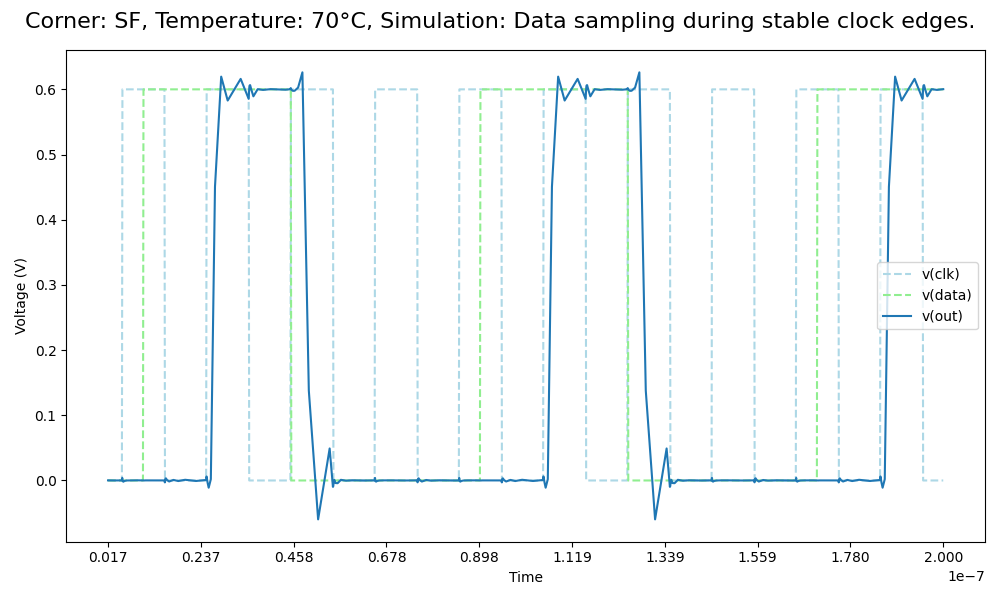
\includegraphics[height= 0.21\textheight]{figures/aimspice/SF/70/W3.csv.png}
    \vspace{5pt}
    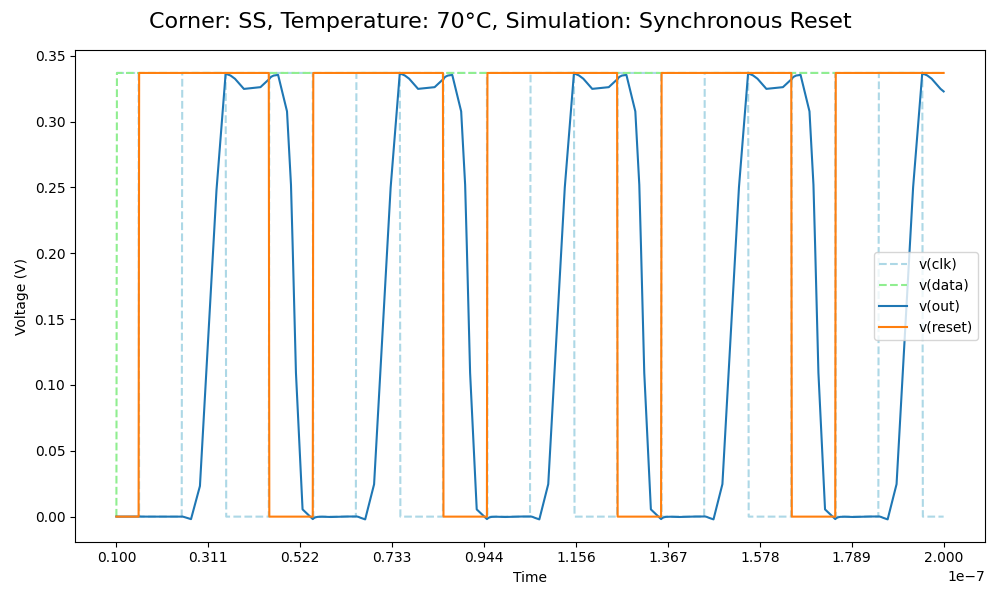
\includegraphics[height= 0.21\textheight]{figures/aimspice/SS/70/W3.csv.png}
    \caption{Simulation of the asynchronous reset at 70 degrees celcius.}
    \label{fig:aimspice_W3_70}
\end{figure}